\documentclass[12pt,twoside,a4paper]{article}
\usepackage{amsmath, amssymb, amsfonts, mathrsfs} %les plus utiles et quasi indispensables 
\usepackage{amsthm}%\usepackage[T1]{fontenc}
\usepackage{a4wide}
\usepackage[utf8]{inputenc}
\usepackage{fancyhdr} %pour les hauts et bas de page
\usepackage[francais]{babel}% donne de bonnes c\'esures  en francais
\usepackage{titlesec}%pour modifier le style des sections
\usepackage{float}%pour fixer les flottants
\usepackage{url}%pour ecrire une adresse d'un site web
\usepackage[all]{xy}%pour faire des diagrammes
\usepackage[dvips]{graphicx}
\usepackage{todonotes}
\usepackage{graphicx}
\usepackage{pgf,tikz}
\usetikzlibrary{arrows}
\usepackage{enumitem}
\usepackage[T1]{fontenc}
\usepackage{hyperref}
\usepackage{array}
\usepackage{chemfig}
\usepackage{graphics}
\usepackage{eurosym}
\usepackage{soul}
\usepackage{wasysym}
\usepackage{textcomp}
\usepackage{listings}
\usepackage{stmaryrd}



\title{TDLog : \textsc{Jelly}}
\author{\textsc{BATY L\'eo, BRUNOD-INDRIGO Luca, CAMPO Yannis,}\\ \textsc{LAURET J\'eremy, LO Emmanuel}}
\date{15/02/2019}


\begin{document}
\maketitle

\tableofcontents

\newpage%%%

L'objectif initial de ce projet \'etait de cr\'eer un jeu multi-joueur en ligne, adaptation d'un jeu de plateau cr\'e\'e l'ann\'ee derni\`ere dans le cadre du cours de d\'eveloppement durable. 

\section{Pr\'esentation du jeu}

Dans ce jeu, les joueurs incarnent chacun un pays. Ils doivent g\'erer le d\'eveloppement \'economique, social, et environemental du pays durant deux \`eres, depuis la r\'evolution industielle jusqu'\`a nos jours. Chaque \`ere se d\'ecompose en tours appel\'es g\'en\'erations, dans lesquels les joueurs jouent simultan\'ement en construisant des b\^atiments, recherchant des technologies et concluant des accords, puis d\`es que tout le monde a valid\'e on passe \`a la g\'en\'eration suivante.\\


\subsection{D\'eroulement d'une g\'en\'eration}
\noindent Chaque g\'en\'eration se d\'eroule en trois phases:

\begin{enumerate}
\item Phase de revenus
\item Phase principale
\item Phase \'ev\`enements
\end{enumerate}

\subsubsection{Phase de revenus}

Chaque joueur poss\`ede trois champs principaux :
\begin{itemize}
\item ses ressources stockables : UM (unit\'e mon\'etaire) et hydrocarbures
\item sa production exc\'edentaire : UM, hydrocarbures, nourriture, pollution, d\'echets, \'electricit\'e, r\'eg\'en\'eration de l'environnement. Par exemple, une production n\'egative de nourriture veut dire que le joueur doit importer les ressources correspondantes afin de satisfaire le besoin de son pays.
\item l'\'etat de son d\'eveloppement : social, \'economique, et environnemental (entier entre 0 et 100)\\
\end{itemize}

Durant la phase de revenus, chaque joueur re\c coit son revenu en UM, doit importer nourriture et \'electricit\'e si ils sont en production n\'egative, ou les exporter si il sont en production positive.\\
Les revenus d'hydrocarbures fonctionnent d'une mani\`ere un peu particuli\`ere. Au d\'ebut de la partie, on constitue trois piles d'hydrocarbures repr\'esentant la r\'eserve mondiale. 

Lorsque l'on produit des hydrocarbures, on ajoute des hydrocarbures aux resources du joueur de la mani\`ere suivante :

\begin{itemize}
\item Tant qu'une pile n'est pas vide on prend les ressources toujours dans la m\^eme zone en commen\c cant par la premi\`ere.
\item Si au d\'ebut de la phase revenus il y avait des ressources dans la pile 1, on prend 3 hydrocarbures par point de production que l'on poss\'ede et on les place dans notre r\'eserve.
\item Si au d\'ebut de la phase revenus la pile 1 \'etait vide et la pile 2 non vide, chaque point de production rapporte 2 hydrocarbures.
\item Si au d\'ebut de la phase revenus les pile 1 et 2 \'etaient vides, chaque point production rapporte 1 ressource.
\item S'il n'y a plus de ressources dans la r\'eserve, on n'en prend pas.
\end{itemize}


\subsubsection{Phase principale}

Durant la phase principale, les joueurs effectuent des actions de mani\`ere simulatn\'ee. Voici la liste des actions possibles :

\begin{itemize}
\item Construire un b\^atiment d\'ebloqu\'e. Chaque b\^atiment a un co\^ut en UM, des modificateurs au niveau de la production du joueur et de son d\'eveloppement, et un \'eventuel effet (ponctuel ou permanent).
\item Acheter une technologie d\'ebloquable. Chaque technologie d\'ebloque une ou plusieurs technologies, un ou plusieurs b\^atiments, et poss\`ede un \'eventuel effet (ponctuel ou permanent).
\item Conclure des accords d'importation ou d'exportation. Chaque accord est propos\'e ou non de mani\`ere al\'eatoire au joueur, et r\'eduit le co\^ut des importations ou permet des exportations d'une ou plusieurs ressources pendant un certain nombre de g\'en\'erations.
\end{itemize}

Chaque joueur peut effectuer autant d'actions qu'il veut, dans la limites des fonds disponibles. Cependant, il ne peut plus construire de b\^atiments d\`es qu'il a construit une technologie, cela simulant que la recherche met du temps \`a devenir effective.

\subsubsection{Phase \'ev\`enements}

A la fin de chaque g\'en\'eration, on tire al\`eatoirement un \'ev\`enement correspondant \`a l'\`ere en cours, et on l'applique \`a tous les joueurs. Les \'ev\`enements ont des effets tr\`es vari\'es d\'ependants de l'\'etat du d\'eveloppement des joueurs. Certains s'appliquent de la m\^eme mani\`ere \`a chaque joueur, et donc regardent la moyenne (ou le minimum/maximum) de chaque \'etat, d'autres s'appliquent individuellement.
La fin de chaque \`ere est d\'eclench\'ee par des \'ev\`enements particuliers appel\'es \'ev\`enements finaux. Ces \'ev\`enements ont des effets plus radicaux que les \'ev\`enements classiques, et d\'eclenchent le d\'ebut de l'\`ere suivante. A la derni\`ere \`ere, l'\'ev\`enement final d\'eclenche un dernier tour sans \'ev\`enements avant la fin de la partie.

\subsection{D\'ecompte des points}

A la fin de la partie on d\'ecompte les points pour chaque joueur. Chaque joueur classe les trois \'echelles de d\'eveloppement dans l'ordre d\'ecroissant de sa position sur ces derni\`eres, et calcule son score de la mani\`ere suivante:

\begin{enumerate}
\item Chaque niveau atteint sur l'\'echelle de d\'eveloppement la plus haute rapporte 1 point.
\item Chaque niveau atteint sur l'\'echelle interm\'ediaire rapporte 2 points.
\item Chaque niveau atteint sur l'\'echelle la plus basse rapporte 3 points.
\end{enumerate}

\noindent Le joueur poss\'edant le plus de points remporte la partie.


\section{Objectifs initiaux}

\noindent Voici la liste des objectifs principaux fix\'es au d\'ebut du projet :

\begin{enumerate}
\item Coder le jeu ainsi que le plus de fonctionalit\'es possibles parmi celles d\'ecrites dans la section pr\'ec\'edente.
\item Y ajouter un syst\`eme qui permet de cr\'eer des parties, d'en rejoindre, d'en lancer, et d'en sauvegarder. 
\item Cr\'eer un site internet h\'ebergeant le jeu
\end{enumerate}

\section{Organisation/architecture du code}

Nous avons utilis\'e un backend en python avec le framework Django, et un frontend Javascript avec la librairie React.

\subsection{Backend Django}

Nous avons cod\'e le backend en Python \`a l'aide du framework Django. Le backend est compos\'e de quatre applications. L'application principale est l'application \textit{game}, dans laquelle se trouve les mod\`eles repr\'esentant les diff\'erents composants du jeu,  les fonctions associ\'ees aux r\`egles du jeu, ainsi l'API django REST framework qui permet le lien avec le frontend \`a l'aide de requ\^etes d'URL.\\

Voici le diagramme UML repr\'esentant les mod\`eles de l'application \textit{game} repr\'esentant une partie ainsi que leur organisation :

\begin{figure}[H]
\centering
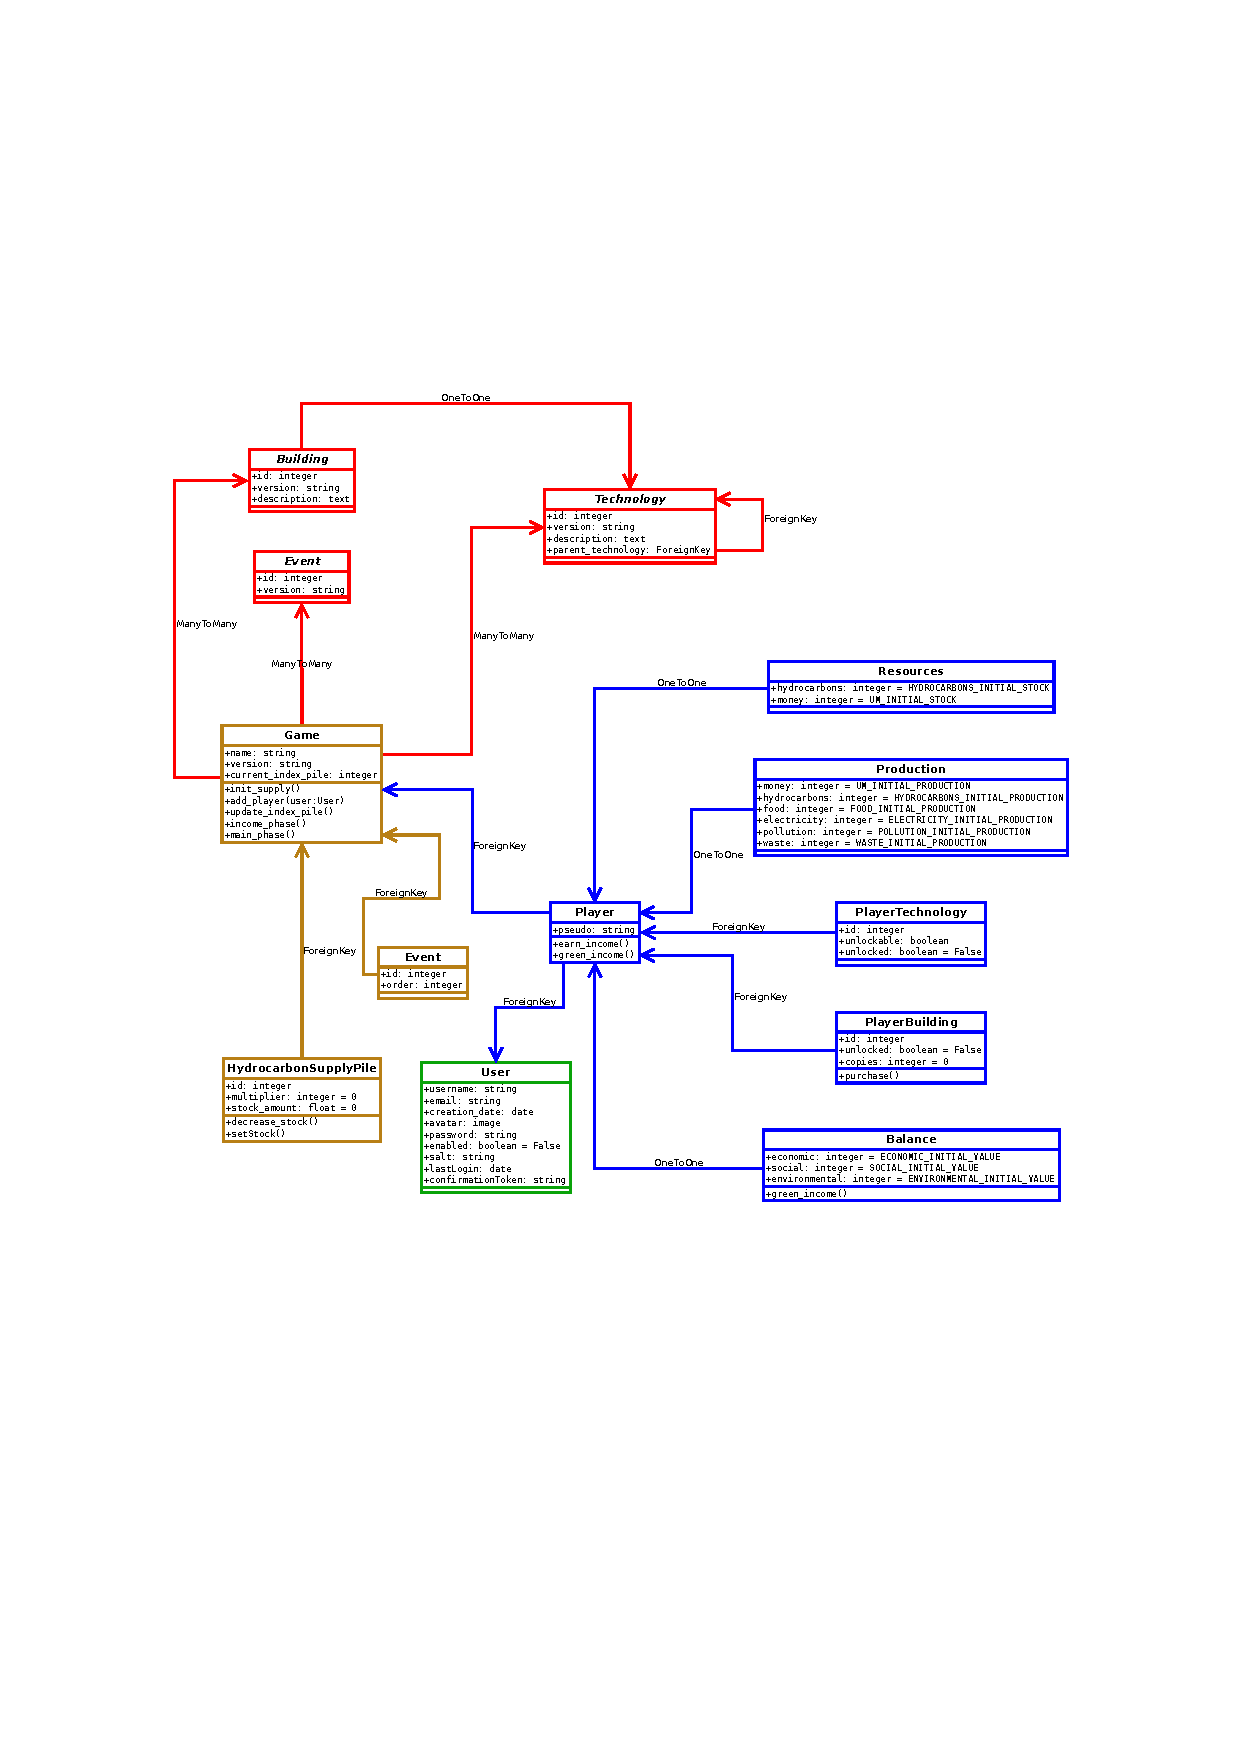
\includegraphics[width=15cm]{../global_uml.pdf}
\caption{Diagramme UML des mod\`eles}
\end{figure}

Comme indiqu\'e sur le diagramme, on a tout d'abord une classe centrale \textbf{Game}, \`a laquelle sont reli\'ees les fixtures (\'ecrites dans des fichiers .json puis charg\'ees en tant qu'instances de mod\`eles) repr\'esent\'ees par les mod\`eles \textbf{SourceBuilding} (b\^atiments), \textbf{SourceTechnology} (technologies), et \textbf{SourceEvent} (\'ev\`enements). Puis, \`a \textbf{Game} sont reli\'es avec une relation ForeignKey (many to one) les mod\`eles \textbf{HydrocarbonSupplyPile} (piles d'hydrocarbures, qui sont ordonn\'ees par leur index) et \textbf{Event} ("deck" d'\'ev\`enemements pour cette partie, ordonn\'ees par leur index, et li\'ees en OneToOne aux SourceEvent). Le deuxi\`eme mod\`ele central de l'architecture du backend est le mod\`ele \textbf{Player} qui est reli\'e \`a \textbf{Game} par une ForeignKey. Chaque \textbf{Player} poss\`ede un \textbf{PlayerState}, auquel sont reli\'es les mod\`eles \textbf{Resources}, \textbf{Production}, \textbf{Balance}, \textbf{Technology}, et \textbf{Building}. De plus, chaque le \textbf{Player} est li\'e \`a un \textbf{ShadowPlayer}, qui est lui m\^eme li\'e \`a un \textbf{PlayerState}. Cela permet d'impl\'ementer la pile d'action : au d\'ebut de la phase principale de chaque joueur, on copie le Player dans le ShadowPlayer, puis pendant toute la phase on effectue les actions sur le ShadowPlayer et on copie \`a nouveau le Player dans le ShadowPlayer \`a chaque annulation des actions. Enfin, \`a la fin du tour un met \`a jour le Player avec le ShadowPlayer.

\subsection{Frontend React}

\section{El\'ements r\'ealis\'es}
\todo[inline]{(il est usuel d'avoir un delta avec les objectifs initiaux)}

\section{Probl\`emes r\'ealis\'es}
\todo[inline]{(afin que nous capitalisions de l'expérience en vue des prochaines promos)}


\end{document}